\chapter{Future Work} 

\section{Future datasets}
The datasets that we used in this dissertation are relatively small---on the order of 10s of different parameter combinations.
The limited scope of these datasets means that we are only able to coarsely cover the entire parameter space.
We hypothesize that we would get better reduced models if we were able to train on larger models.
Generating large biological datasets by hand is difficult and error prone.
However, we demonstrated the potential for further lab automation by generating a dataset using the Labcyte Echo liquid handler.
We encourage future work to take this even further and generate datasets with hundreds or even thousands of starting conditions.
Another logical extension is to use datasets generated from organisms other than \gls{ecoli}.

\begin{figure}[t!]
\begin{center}
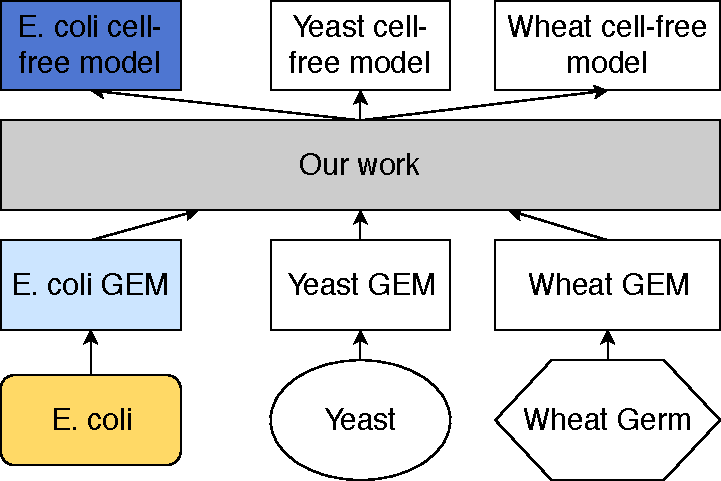
\includegraphics{figs/Vision.pdf}
\caption[Our system can generate cell-free models for any organism]
{Our system was designed to convert any organism's \glspl{gem} into an appropriate cell-free model.
}
\end{center}
\label{fig:vision}
\end{figure}

\section{Different Organisms}
This work has only explored the generation of \gls{ecoli} cell-free models.
However, much ongoing work involves the use of non-\gls{ecoli} organisms.
This system was written in such a way that it can be applied to any organism with a \gls{gem}.
Figure \ref{fig:vision} demonstrates our vision of how our system could be used in the future.
Instead of creating a model by hand that only describes our \gls{cfps} system, our system can now be used to create cell-free metabolic models for many different organisms.
In particular, the primary author of this work is a part of an OpenPlant grant involving modeling wheat-germ cell-free systems.
The data is currently being generated, and we plan to apply our system to this new \gls{cfps} system as soon possible.
%TODO add/explain?
%Additionally, this system will get a web interface to encourage other biologists to use it for their own data.
%TODO: talk about https://www.cell.com/cell-systems/pdf/S2405-4712(17)30010-8.pdf

One issue is that this pipeline is only as good as the initial models.
The initial \gls{fba} model is an imperfect description of a full \gls{ecoli} cell, so any errors in that overall model will be replicated in our reduced models.
\gls{fba} models are periodically updated with new data.
Our system is built to be flexible and can easily produce new models based on any updates.

\section{RL system for reduction}
Our use of a \gls{vae} as a dimensionality reduction tool proved to be quite powerful, but the part of the system that converted from the reduced representation back into a \gls{fba} model was quite simple.
We removed reactions based on a simple thresholding criterion.
Instead of deciding which reactions to remove using a threshold, we could reframe this problem as a reinforcement learning problem.
Using a combination of experimental data, a starting \gls{fba} model, and a latent representation of the problem space, more sophisticated search methods could likely produce better reduced models.
To that end, we also provide a framework built on top of OpenAI's Gym environment for performing reinforcement learning on \gls{fba} models.
Given a starting model with almost 2600 reactions, the space of possible reduced models is enormous.
Thus, we believe a combination of our Corr-VAE and reinforcement learning could yield a better reduced model.

\begin{figure}[t!]
\begin{center}
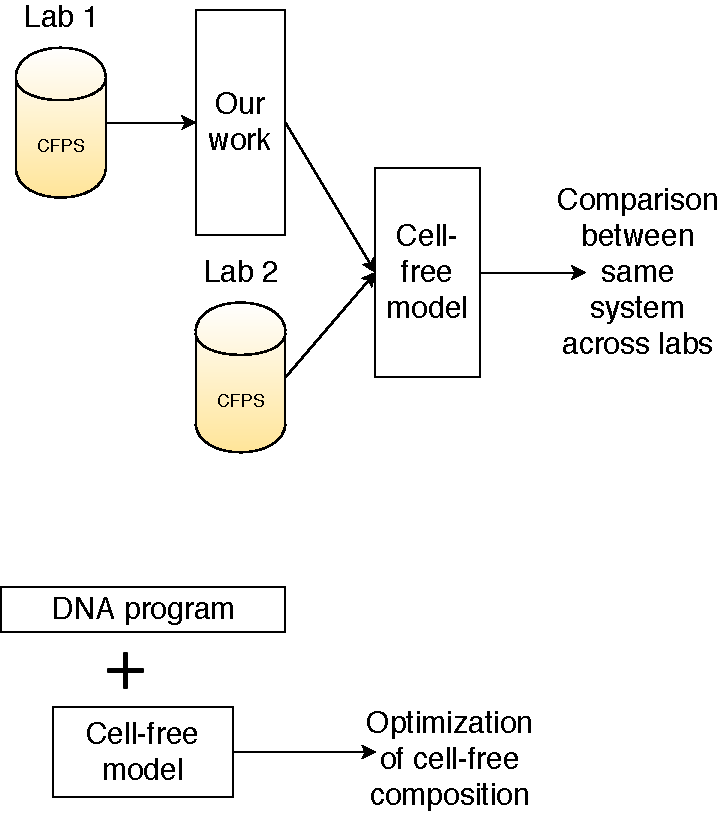
\includegraphics{figs/Applications.pdf}
\caption[Future applications for our system]
{Two future applications of our system.
Above, multiple experiments can be projected in the same subspace to better compare experimental results.
Below, the system can help optimize the energetic composition of a cell-free system}
\end{center}
\label{fig:apps}
\end{figure}

\section{Batch variation}
Finally, we envision an important use for our system as a way of dealing with batch variation in \gls{cfps} systems.
Batch variation is an important problem facing the cell-free community~\cite{sun2013protocols, chizzolini2017cell}.
The current solution to this problem is to run everything that needs to be compared in the same batch.
This is problematic, though, if the batch runs out or someone else wants to reproduce this result.
The only way to deal with this problem would be to redo all of the experiments in a new batch.

Figure \ref{fig:apps} shows how our system provides a potential solution to this issue of batch variation.
A researcher runs a calibration set of experiments and then uses those experimental results to generate a \gls{vae} model.
Now, this \gls{vae} can be used to project any future experimental into the same latent space as the first set of experiments.
These experiments could be compared within the latent space, or they could be transformed back into the original dimensionality of the data.
This transformed data should allow for better comparisons across batches.

% Generative nature of VAEs
% Can generate "typical" fluxes for a subspace
% Traverse the subspace 